\documentclass[journal]{IEEEtran}

% correct bad hyphenation here
\hyphenation{}

%Import packages
\usepackage{amsmath}
\usepackage{listings}
\usepackage[utf8]{inputenc}
\usepackage{algpseudocode}
\usepackage{algorithm}
\usepackage[]{hyperref}
\usepackage{url}
\usepackage{pgfgantt}
\usepackage{comment}
\usepackage{array}
\usepackage[section]{placeins}
\usepackage{array,xstring}
\usepackage{numprint} 
\usepackage{pdflscape} %%landscape
\usepackage{rotating}
\usepackage{graphicx}
\usepackage{caption}
\usepackage{varwidth}

\DeclareCaptionFormat{myformat}{%
  % #1: label (e.g. "Table 1")
  % #2: separator (e.g. ": ")
  % #3: caption text
  \begin{varwidth}{\linewidth}%
    \centering
    #1#2#3%
  \end{varwidth}%
}


%%COMANDOS
\newcommand{\writetable}[5]{ %numerocaso,algoritmo, pc, pm, numind
\captionsetup{format=myformat, labelsep=newline}

\subsection{Caso #1:}
\begin{table}[!htb]
\begin{center}
  \begin{tabular}{|l | r | r | N{5}{4} | n{5}{4} | n{5}{4} | N{5}{4} | l|}
  \hline

  \multicolumn{1}{|l}{Instancia}&
  \multicolumn{1}{|c}{$F_{OPT}$}&
  \multicolumn{1}{|c}{$F_{BEST}$}&
  \multicolumn{1}{|c}{$F_{AVG}$}&
  \multicolumn{1}{|c}{$\sigma$}&
  \multicolumn{1}{|c}{$T_{AVG}$}&
  \multicolumn{1}{|c}{$DA$}&
  \multicolumn{1}{|c|}{Normal}\tabularnewline
  \hline

  \input{./tablas/tabla#1-#2.tex}

  \hline
  \end{tabular}
\end{center}

\IfEqCase{#2}{%
        {GA}{
        \caption{
        $P_{C}=#3, P_{M}=#4, \#Individuos=#5$ \newline
        (*) $\sigma=0$  No definido DA, se asume Normalidad.}
        }
        {CHC}{
        \caption{
        $P_{C}=#3, P_{R}=#4 , \#Individuos=#5$ \newline
        (*) $\sigma=0$  No definido DA, se asume Normalidad.}
        }
        % you can add more cases here as desired
    }

\end{table}

}

\hypersetup{
    pdftitle={Job Shop Scheduling},
    %pdfauthor={Your name here},
    %pdfsubject={Your subject here},
    %pdfkeywords={keyword1, keyword2},
    bookmarksnumbered=true,     
    bookmarksopen=true,         
    bookmarksopenlevel=1,       
    colorlinks=true,            
    pdfstartview=Fit,           
    pdfpagemode=UseOutlines,    % this is the option you were lookin for
    pdfpagelayout=TwoPageRight,
    urlcolor=blue,
    linkcolor=blue,
    citecolor=red
}

\newcommand{\writetableBest}[5]{ %numerocaso,algoritmo, pc, pm, numind
\captionsetup{format=myformat, labelsep=newline}

\subsection{Caso 5000 Generaciones:}
\begin{table}[!htb]
\begin{center}
  \begin{tabular}{|l | r | r | N{5}{4} | n{5}{4} | n{5}{4} | N{5}{4} | l|}
  \hline

  \multicolumn{1}{|l}{Instancia}&
  \multicolumn{1}{|c}{$F_{OPT}$}&
  \multicolumn{1}{|c}{$F_{BEST}$}&
  \multicolumn{1}{|c}{$F_{AVG}$}&
  \multicolumn{1}{|c}{$\sigma$}&
  \multicolumn{1}{|c}{$T_{AVG}$}&
  \multicolumn{1}{|c}{$DA$}&
  \multicolumn{1}{|c|}{Normal}\tabularnewline
  \hline

  \input{./tablas/tabla#1-#2.tex}

  \hline
  \end{tabular}
\end{center}

\IfEqCase{#2}{%
        {GA}{
        \caption{
        $P_{C}=#3, P_{M}=#4, \#Individuos=#5$ \newline
        (*) $\sigma=0$  No definido DA, se asume Normalidad.}
        }
        {CHC}{
        \caption{
        $P_{C}=#3, P_{R}=#4 , \#Individuos=#5$ \newline
        (*) $\sigma=0$  No definido DA, se asume Normalidad.}
        }
        % you can add more cases here as desired
    }

\end{table}

}



\newcommand{\writetablecases}{

\begin{table}[]%!ht
 \begin{center}
 \scalebox{0.6}{
  \begin{tabular}{|l|l|l|l|l|n{5}{4}|n{5}{4}|n{5}{4}|n{5}{4}|}
  \hline
   
  \multicolumn{1}{|l}{Instancia}&
  \multicolumn{1}{|c}{}&
  \multicolumn{1}{|c}{}&   
  \multicolumn{1}{|c}{}&
  \multicolumn{1}{|c}{}&    
  \multicolumn{2}{|c|}{GA}&
  \multicolumn{2}{c|}{CHC}
  \tabularnewline

  \multicolumn{1}{|l}{}&
  \multicolumn{1}{|l}{$P_{C}$}&
  \multicolumn{1}{|l}{$P_{M}$}&
  \multicolumn{1}{|l}{$\#ind$}&
  \multicolumn{1}{|l}{$P_{R}$}& 
  \multicolumn{1}{|c}{$F_{AVG}$}&
  \multicolumn{1}{c|}{$T_{AVG}$}&
  \multicolumn{1}{c}{$F_{AVG}$}&
  \multicolumn{1}{c|}{$T_{AVG}$}
  \tabularnewline
  \hline
  
  1 & 0.6 & 0.01 & 50 & 878.0416666666666 & 5.759520166666666 & 1006.585 & 26.70969613333333\tabularnewline
2 & 0.6 & 0.01 & 100 & 877.875 & 6.260110599999999 & 1006.203333333333 & 27.28910808333332\tabularnewline
3 & 0.6 & 0.01 & 200 & 878.6650000000002 & 6.595528383333334 & 1004.673333333333 & 26.80654705\tabularnewline
4 & 0.7 & 0.01 & 50 & 879.2966666666667 & 6.228625033333334 & 982.2283333333331 & 53.57978788333334\tabularnewline
5 & 0.8 & 0.01 & 50 & 878.0549999999999 & 6.577643533333334 & 983.0483333333334 & 54.42023520000001\tabularnewline
6 & 0.6 & 0.05 & 50 & 879.325 & 6.550134866666665 & 984.1066666666666 & 52.37533545\tabularnewline
7 & 0.7 & 0.05 & 50 & 879.9716666666669 & 6.68282325 & 982.2283333333331 & 53.57978788333334\tabularnewline
8 & 0.8 & 0.05 & 50 & 880.5783333333333 & 6.5200783 & 983.0483333333334 & 54.42023520000001\tabularnewline
9 & 0.6 & 0.1 & 50 & 879.1966666666665 & 5.925307466666666 & 984.1066666666666 & 52.37533545\tabularnewline
10 & 0.7 & 0.1 & 50 & 880.8800000000001 & 6.178663999999999 & 982.2283333333331 & 53.57978788333334\tabularnewline
11 & 0.8 & 0.1 & 50 & 879.0283333333331 & 7.103025050000001 & 983.0483333333334 & 54.42023520000001\tabularnewline
12 & 0.7 & 0.01 & 100 & 880.6216666666666 & 5.874728616666667 & 984.1066666666666 & 52.37533545\tabularnewline
13 & 0.8 & 0.01 & 100 & 882.5150000000001 & 6.36609365 & 961.1599999999999 & 108.11545685\tabularnewline
14 & 0.6 & 0.05 & 100 & 882.835 & 6.867328066666667 & 962.8749999999998 & 106.0741529\tabularnewline
15 & 0.7 & 0.05 & 100 & 882.85 & 6.6304395 & 962.8699999999999 & 103.77437405\tabularnewline
16 & 0.8 & 0.05 & 100 & 882.7316666666666 & 6.823273666666667 & 961.1599999999999 & 108.11545685\tabularnewline
17 & 0.6 & 0.1 & 100 & 881.6966666666667 & 7.360386666666668 & 962.8749999999998 & 106.0741529\tabularnewline
18 & 0.7 & 0.1 & 100 & 882.3616666666669 & 6.37960635 & 962.8699999999999 & 103.77437405\tabularnewline
19 & 0.8 & 0.1 & 100 & 882.3800000000001 & 6.62577535 & 961.1599999999999 & 108.11545685\tabularnewline
20 & 0.7 & 0.01 & 200 & 881.9483333333334 & 6.633349716666666 & 962.8749999999998 & 106.0741529\tabularnewline
21 & 0.8 & 0.01 & 200 & 880.6633333333333 & 5.971453700000002 & 962.8699999999999 & 103.77437405\tabularnewline
22 & 0.6 & 0.05 & 200 & 879.1566666666668 & 6.234902516666667 & 1006.203333333333 & 27.28910808333332\tabularnewline
23 & 0.7 & 0.05 & 200 & 877.1283333333331 & 6.5125129 & 1004.673333333333 & 26.80654705\tabularnewline
24 & 0.8 & 0.05 & 200 & 877.8416666666666 & 5.921532233333332 & 1006.585 & 26.70969613333333\tabularnewline
25 & 0.6 & 0.1 & 200 & 879.2433333333332 & 6.1109201 & 1006.203333333333 & 27.28910808333332\tabularnewline
26 & 0.7 & 0.1 & 200 & 879.2066666666667 & 6.687247483333333 & 1004.673333333333 & 26.80654705\tabularnewline
27 & 0.8 & 0.1 & 200 & 879 & 5.899790949999998 & 1006.585 & 26.70969613333333\tabularnewline

  
  \hline
  \end{tabular}
  }
\end{center}
\caption{Ajuste de parámetros}
\label{tabla:todoscasos}
\end{table}

}

\newcommand{\writetableglobal}[4]{

\begin{table}[!ht]
\begin{center}
  \begin{tabular}{|l|r|r|n{5}{4}|n{5}{4}|n{5}{4}|n{5}{4}|n{5}{4}|n{5}{4}|n{5}{4}|n{5}{4}|l|l|}
  \hline
  \multicolumn{1}{|l}{}&
  \multicolumn{2}{|c}{$F_{BEST}$}&
  \multicolumn{2}{|c}{$F_{AVG}$}&
  \multicolumn{2}{|c}{$\sigma$}&
  \multicolumn{2}{|c}{$T_{AVG}$}&
  \multicolumn{2}{|c}{DA}&
  \multicolumn{2}{|c|}{Normal}
  \tabularnewline

   
  \multicolumn{1}{|l}{Instancia}&
  \multicolumn{1}{|c}{GA}&
  \multicolumn{1}{c}{CHC}&
  \multicolumn{1}{|c}{GA}&
  \multicolumn{1}{c}{CHC}&
  \multicolumn{1}{|c}{GA}&
  \multicolumn{1}{c}{CHC}&
  \multicolumn{1}{|c}{GA}&
  \multicolumn{1}{c}{CHC}&
  \multicolumn{1}{|c}{GA}&
  \multicolumn{1}{c}{CHC}&
  \multicolumn{1}{|c}{GA}&
  \multicolumn{1}{c|}{CHC}
  \tabularnewline
  \hline
  
  \input{./tablas/tabla#1-GA-CHC.tex}
  
  \hline
  \end{tabular}
  
\end{center}
\caption{$P_{C}=#2, P_{M}=#3, \#Individuos=#4$}
\end{table}

\newpage
}



\begin{document}
\title{Job Shop Scheduling\\ Algoritmos Evolutivos\\ Grupo 12}


\author{
Sergio~Bonilla, 4.430.955-3\\
Leonardo~Clavijo, 5.054.830-5\\
\{serginhobonilla, joleocl\}@gmail.com
}

% The paper headers
\markboth{Job Shop Scheduling, Algoritmos Evolutivos 2014}%
{Shell \MakeLowercase{\textit{et al.}}: Bare Demo of IEEEtran.cls for Computer Society Journals}


\IEEEtitleabstractindextext{%
\begin{abstract}
Este artículo presenta un algoritmo evolutivo eficiente aplicado al problema Hard-NP conocido como Job Shop Scheduling. El algoritmo planteado está especialmente diseñado para lograr soluciones óptimas al problema, utilizando operadores evolutivos específicos, y una codificación que impacta de forma positiva generando soluciones factibles al problema. En la sección evaluación experimental se plantea las acciones a tomar para demostrar la eficiencia del algoritmo ante versiones deterministas que resuelven el problema utilizando heurísticas simples. Se plantea la comparación entre operadores de cruzamiento y el impacto que puede tener éste sobre la calidad de la solución al problema. El objetivo es brindar una solución eficiente a JSSP utilizando algoritmos evolutivos, mejorando resultados obtenidos a partir de heurísticas.
\end{abstract}
}

\maketitle

\IEEEdisplaynontitleabstractindextext

\IEEEpeerreviewmaketitle


\section{Introducción}
En el siguiente trabajo se presentará un problema de optimización combinatoria como es la planificación de procesos en un ambiente multiprocesador. Se explicará acerca de las técnicas utilizadas resolver el problema. Se hará una presentación formal acerca de éste y se compararán resultados con respecto a otras modalidades de resolución.

\section{Algoritmos Evolutivos}
La computación evolutiva es una rama de la computación; y en particular de la inteligencia artificial. Se la puede definir como un conjunto de metaheurísticas que emulan la evolución biológica. Interpretando a la naturaleza e inspirados en la teoría de la evolución de Charles Darwin, se crea un mecanismo análogo a los procesos evolutivos de ésta, con el objetivo primordial de resolver problemas de optimización combinatoria. 
	Este mecanismo trabaja con una población de individuos, que sigue la idea de supervivencia de los individuos más aptos (mediante una función de fitness), la idea de reproducción (mutación y recombinación) y la idea de diversidad genética.


\section{Job Shop Scheduling}
Uno de los problemas clásicos dentro del área de ciencias en computación y la optimización combinatoria, es el problema conocido como JSP (Job Shop Scheduling). 	Los problemas de optimización combinatoria, básicamente poseen un espacio de soluciones discretas, pero que en general son muy grandes debido a que se representan como permutaciones o combinaciones. Por lo que encontrar una solución óptima, o cercana a él, es bastante complejo con técnicas comunes. 
	Este tipo de problemas se los caracteriza como difíciles o NP-difíciles. Es por eso que se decide utilizar técnicas de algoritmos evolutivos para plantear una posible solución al JSP.

	El problema de Job Shop Scheduling  es un tipo de problema de planificación de tareas, y en particular de optimización; donde se busca optimizar el makespan o tiempo de ejecución de todas las tareas. 
	Básicamente el problema consiste en planificar un conjunto de tareas (Jobs) N sobre un conjunto de recursos o máquinas heterogéneas M. 
	Por otra parte se tiene que cada Job está compuesto por un conjunto de operaciones, las cuales son dependientes, es decir, se deben ejecutar en forma secuencial. 
	Además cada tarea tiene un tiempo de término más tardío, no hay restricciones de precedencia entre operaciones de distintas tareas y el planificador es no expropiativo.
	
	El problema queda definido de la siguiente forma:
\begin{itemize}
  \item Se considera un conjunto de $N$ tareas, independientes entre ellas.
  \item Sea $M$ la cantidad de máquinas involucradas en el problema, presentan la característica de ser heterogéneas, capaces de ejecutar únicamente una tarea por vez.
  \item Un trabajo $j, 1\leq j \leq J$  está compuesto por $K_{j}$ operaciones.
  \item Las operaciones mantienen un orden de precedencia preestablecido, esto quiere decir $o_{j,1}\le o_{j,2} \le ... \le o_{j,K_{j}}$.
  \item No existe dependencias entre operaciones de distintas tareas.
  \item Existen tiempos de ejecución predefinidos dado un trabajo $j$, una operación $k$ y una máquina $m$, se define en una matriz costos $C_{j,k,m}$, con $1\leq j \leq J, 1\leq k \leq K_{j}, 1\leq m \leq M$.
  \item Planificador no expropiativo, esto se debe a que las tareas poseen tiempo de término máximo, por lo cual no puede expropiarse el recurso a una operación una vez le es asignado el recurso.
  \item Se desea obtener el tiempo de comienzo de ejecución para cada operación, y en qué máquina son asignadas las mismas. Para ello se define $t_{j,k,m}$ como el tiempo de inicio de ejecución de la operación $o_{j,k}$ en la máquina $m$. Por lo cual para cada operación se obtendrá el par $(t_{inicio}, m)$.
\end{itemize}

Una vez definido el problema en cuestión, se procede a la formulación matemática del mismo, esto implica la función objetivo a optimizar, en conjunto con las restricciones del problema planteadas en el punto anterior.

El objetivo es minimizar el makespan. Estas son las variables utilizadas para la formulación:
\begin{itemize}
  \item $t_{j,k,m}$: tiempo de inicio de ejecución de la operación $k$ correspondiente al trabajo $j$ en la máquina $m$.
  \item $C_{j,k,m}$: tiempo de proceso de la operación $k$ del trabajo $j$ en la máquina $m$.
  \item $p_{j',k',j,k,m}$: variable binaria que define si una operación precede a otra \[
p_{j',k',j,k,m}
\begin{cases}
    1,& \text{ $(j,k)$ anterior a $(j',k')$ en $m$ } \\
    0,              & \text{otro caso}
\end{cases}
\]

\item $M$: Número positivo.
\end{itemize}


La formulación matemática queda definida:\\

Minimizar makespan
\begin{equation}
\label{eq1}
  f: min \{ max\{t_{j,K_{j},m}+C_{j,K_{j},m}\} \}
\end{equation}

s.a

%restriccion sobre precedencia tarea
\begin{equation}
\label{eq2}
  t_{j,k,m} + C_{j,k,m} \leq t_{j,k+1,m} \forall j,k,m
\end{equation}


\begin{equation}
\label{eq4}
   t_{j,k,m} + C_{j,k,m} \leq t_{j',k',m} + M \cdot (1- p_{j',k',j,k,m}) \forall j,j',k,m
\end{equation}

\begin{equation}
\label{eq5}
   t_{j',k',m} + C_{j',k',m} \leq t_{j,k,m} + M \cdot p_{j',k',j,k,m} \forall j,j',k,m
\end{equation}

\begin{equation}
\label{eq6}
  t_{j,k,m} \geq 0   \forall j,k,m
\end{equation}

\begin{equation}
\label{eq8}
  C_{j,k,m} \geq 0 \forall j,k,m
\end{equation}
Donde $1 \leq j,j' \leq J$, $J$ cantidad de trabajos del problema; $1 \leq m \leq M$, siendo $M$ la cantidad de máquinas del problema; $K_{j}$ la cantidad de operaciones de la tarea $j$; $1\leq k,k' \leq K_{j}$.
La ecuación \eqref{eq1} es la función objetivo del problema.
En la ecuación \eqref{eq2} se impone restricción sobre la precedencia de las operaciones. 

En las ecuaciones \eqref{eq4} y \eqref{eq5} se impone restricción sobre la utilización de la máquina, una máquina procesa una operación a la vez.
En las ecuaciones \eqref{eq6} y \eqref{eq8} define que las variables en cuestión deben ser positivas.


\newpage


\section{Estrategia de Resolución}
En esta subsección se describirán los operadores evolutivos a utilizar, la codificación del problema y la función fitness.


\subsection{Codificación}
Existen dos categorías de codificar un problema, la representación directa \cite{url:rep}\cite{url:repdirecta} refiere a codificar el cromosoma como el problema en sí mismo, mientras que la representación indirecta recurre a una estructura distinta, sea por motivos de eficiencia o complejidad de la solución.
La codificación seleccionada es indirecta, consiste en una estructura $M$ con un arreglo de tamaño $\sum_{i=1}^{J} cantidad\_operaciones(J)$ representando la cantidad total de operaciones involucradas en el problema, para cada celda de la estructura $M$ corresponde a un valor $j, 0\leq\ j \leq J$, donde $J$ es la cantidad del trabajos. De esta forma se obtiene el orden de las operaciones a ser ejecutadas. Observar que se cumple las restricciones del problema, ya que las operaciones dentro de una tarea quedan ordenadas según las ocurrencias en el vector.
Seleccionar correctamente la codificación del problema repercute de forma directa la eficiencia de la solución al problema. La selección de esta estructura parece agregar simplicidad en el momento de resolver el problema, ya que el mismo presenta características deseables en cuanto a las restricciones del problema. Para lograr este objetivo es necesario una estructura que almacene la cantidad de operaciones para cada trabajo, se utiliza un arreglo de tamaño $J$ con la cantidad máxima de operaciones para cada trabajo.
Observar que la codificación seleccionada simplifica el proceso de aplicar operadores evolutivos, tanto primario como ser el cruzamiento como la mutación. Para el caso del cruzamiento basta seleccionar un operador de recombinación de dos puntos, se ha seleccionado éste operador con la idea de mantener el orden preestablecido dada una solución al problema. Si bien este operador genera una solución que no satisface las restricciones del problema, se crea una operación extra [\ref{sec:verif-fact}] para lograr que la solución generada sea satisfactible. De esta forma se fuerza que todas las soluciones al problema sean satisfactibles; este aspecto de forzar a soluciones satisfactibles presenta una característica deseable; la solución al problema converge de forma más rápida.\cite{url:binaria}
También dada la codificación de la solución, se simplifica el operador evolutivo de mutación, seleccionando una celda de forma aleatoria del arreglo y cambiando su valor por una tarea del problema. Posteriormente se requiere un proceso de transformación a una solución satisfactible.


%%referencia Baghi et al., 1991; Bruns, 1993; Uckun et al., 1993

\subsection{Función Fitness}
El objetivo de la función fitness es minimizar el tiempo de finalización de todos los trabajos, se define el tiempo de finalización de cada trabajo como $t_{final}(j,K_{j}) = t_{inicial}(j,K_{j})+C_{j,K_{j},m}$, donde $m$ es el identificador de la máquina que ejecuta la operación $K_{j}$ del trabajo $j$; $C_{j,K_{j},m}$ es el costo asociado dado un trabajo, operación y máquina, de aquí en adelante se representa a una operación de un trabajo $j$ como $o_{j,k} , 1\leq k\leq K_{j}$ donde $K_{j}$ es la cantidad de operaciones del trabajo.
La función fitness será el mayor valor del tiempo de finalización del conjunto de trabajos.


Sea $S$ una solución al problema, la función fitness de $S$ queda expresada \eqref{fitnessfunction}.
\begin{equation}
f(S)= max\{t_{inicial}(j, K_{j}) + C(j,K_{j},m))\} 
\label{fitnessfunction}  
\end{equation}

JSSP se trata de un problema combinatorio, dada la codificación planteada se debe implementar operadores evolutivos específicos para generar soluciones factibles a las restricciones del problema.


\subsection{Inicialización}
\label{sec:init}
En este caso se debe tener en cuenta que inicializar poblaciones de forma aleatoria puede generar soluciones no factibles al problema, para ello se debe implementar un operador de construcción aleatorio, teniendo en cuenta varias heurísticas para obtener una población inicial satisfactible y de ésta forma lograr la convergencia en una solución óptima en menor cantidad de generaciones.
Para generar una población inicial se puede utilizar alguno de los métodos descriptos a continuación:

\begin{enumerate}
    \item Generación aleatoria de individuos, para ello se asigna un valor inicial y luego se le asigna a cada operación una máquina de forma aleatoria, en el transcurso de la operación se debe tener en cuenta las restricciones de dominio sobre los individuos, descriptos en la descripción del problema. Se brindan mecanismos de reparación y checkeo de las soluciones generadas.
  \item Utilizar heurísticas conocidas para la generar una solución al problema, y posteriormente aplicar operadores evolutivos como ser cruzamiento y mutación para generar nuevos individuos.
  \item Priorizar políticas y heurísticas que pueden impactar de forma positiva en la generación de individuos, como ser:
  \begin{itemize}
    \item SPT Shortest Processing Time: Aplicado a las operaciones con menor tiempo de procesamiento y respetando las restricciones de ordenamiento entre operaciones.
    \item LPT Longest Processing Time: Asigna operaciones por mayor tiempo de procesamiento, respetando el orden de ejecución de cada operación.
    \item LMB Load Machine Balance: Brindar mayor prioridad a las operaciones que permitan un mejor balance de la utilización de las máquinas. Esto es útil para no adjudicar operaciones únicamente a las máquinas con mejor performance, de esta forma se logra reducir el tiempo final de ejecución.
  \end{itemize}
\end{enumerate}
Para lograr mayor diversidad en la población, los valores serán creados de forma aleatoria; posteriormente se procede a la reparación del individuo en lo que refiere el tiempo de inicio de ejecución para cada operación.


\subsection{Selección}
Método de selección por torneo, de esta forma se eliminan las soluciones con valores de fitness no deseables, la diversidad se logra aplicando operadores evolutivos, de recombinación como de mutación. 


\subsection{Explotación: Recombinación}
Para realizar el proceso de recombinación, se seleccionan dos padres $A=(A^{1},A^{2},..,A^{K})$ y $B=(B^{1},B^{2},..,B^{K})$, donde $K=\sum_{j=0}^{J}cantidad\_operaciones(j)$ según el método de selección propuesto en el ítem anterior. El operador de recombinación consiste en seleccionar de forma aleatoria dos trabajos $i$ y $j$, con $i \leq j$, y recombinamos los hijos de forma tal que $C=(A^{1},..A^{i-1},B^{i},..,B^{j},A^{j},..,A^{K})$ y de forma análoga procedemos para el segundo hijo $C=(B^{1},..B^{i-1},A^{i},..,A^{j},B^{j},..,B^{K})$.
Recordar que cada trabajo $h$ posee $K_{h}$ operaciones, dada la codificación se obtiene que $M_{h, x_{h}}$ es de la forma $(M_{i},t_{inicial})$ por lo tanto cuando aplicamos el operador de recombinación debemos tener en cuenta el primer término y recalcular el segundo luego de finalizada la operación, se obtienen individuos que cumplen con las restricciones del problema propuesto.
Se presenta un pseudocódigo para la solución del operador recombinación.
\\
\begin{algorithmic}
  \State $S_1= select(S)$
  \State $S_2= select(S)$
  \State $i\gets random(1,K)$
  \State $j \gets random(1,K)$
  
  \For{$c=i$ to $j$}
  \State {$swap \gets S_1[c]$}
  \State {$S_1[c] \gets S_2[c]$}
  \State {$S_2[c] \gets swap$} 
  \EndFor
  
  \State $repair(S_1)$
  \State $repair(S_2)$
\end{algorithmic}



\subsection{Exploración: Mutación}
\label{subsec:mutacion}
Si bien en la propuesta inicial se mencionó la implementación de dos operadores de mutación, se realizó la implementación de un operador específico, puesto que el algoritmo a comparar no presenta operador secundario, se considera oportuno que la implementación de un operador es suficiente para brindar diversidad al problema.
Explorar es un proceso importante para generar diversidad en el conjunto de soluciones, para este caso se implementa un operador de mutación aleatorio que brinda mejoras tanto a nivel de calidad de la solución como eficiencia computacional, dado que el proceso es sencillo de implementar y eficiente computacionalmente hablando, además de agregar diversidad al problema. El operador de mutación en cuestión se representa de la siguiente forma:

\begin{enumerate}
  \item Seleccionar dos operaciones $i,j , 0 \leq j,i \leq K, i\neq j$, con $K=\sum_{j=1}^{J}cantidad\_operaciones(j)$.
  \item Intercambiar el valor de trabajo de las celdas anteriormente seleccionadas.
  \item Reparar la solución, de forma de que sea factible para el problema en cuestión.
\end{enumerate}

Observar que al aplicar el operador de mutación el nuevo individuo cumple con las restricciones de ordenamiento, se aplica mecanismos de reparación y verificación para recalcular los tiempos de inicio de ejecución de cada operación de modo tal que se evita que en una máquina se ejecutan dos procesos al mismo tiempo.

El planteo para la mutación se puede apreciar con el pseudocódigo a continuación:
\\

\begin{algorithmic}
  \State $i \gets random(1,K)$
  \State $j \gets random(1,K)$
  \State $swap \gets S_1[i]$
  \State $S_1[i] \gets S_1[j]$
  \State $S_1[j] \gets swap$
  \State $repair(Mutation)$
\end{algorithmic}

Observar la simplicidad del operador de mutación, computacionalmente es eficiente, se obtienen resultados que satisfacen los requerimientos en cuanto a performance. Brinda diversidad al problema, con lo cual en conjunto con el método de solución y el operador de recombinación la convergencia a una solución óptima ocurre de forma inmediata.

\subsection{Verificación factibilidad y mecanismo de reparación}
\label{sec:verif-fact}
Si bien los operadores de recombinación y mutación no generan soluciones no factibles desde el punto de vista del orden de ejecución de las operaciones, se debe reparar los tiempos de inicio de ejecución para cada operación una vez se ha aplicado mutación/recombinación. 

A continuación se presenta el 'pseudocódigo' relativo al mecanismo de reparación, $Dline_{Jobs}$ y $Dline_{Mach}$ son vectores auxiliares que contienen el tiempo de deadline de los trabajos y máquinas respectivamente.
\\

\begin{algorithmic}
\State $Dline_{Jobs} \gets \vec{0}$
\State $Dline_{Mach} \gets \vec{0}$
\State $i \gets 1$
  \For{$i \leq I$}  
    \State $j \gets 1$
    \For {$j \leq J$}
      \State $Mach \gets machine(M_{j,i})$
      \If {$Dline_{Jobs}[j]>Dline_{Mach}[Mach]$}
        \State $M_{j,i} \gets (Mach, Dline_{Jobs}[j])$
      \Else
        \State $M_{j,i} \gets (Mach,Dline_{Mach}[M]$
      \EndIf     
      \State $Dline_{Jobs}[j]+=C_{j,i,Mach}$ 
      \State $Dline_{Mach}[Mach]+=C_{j,i,Mach}$    
    \EndFor
    \EndFor 
\end{algorithmic}

Observar el orden de ejecución, se debe recorrer todas las operaciones para garantizar la reparación de la solución, si bien resulta un mecanismo costoso también se debe tener el cuenta que la mutación es un operador secundario en la implementación del problema, con lo cual la probabilidad de utilizar este operador es menor, lo cual implica que el costo al aplicar la reparación es despreciable para ese caso.

\subsection{Características CHC}
Brevemente se describe las características del algoritmo CHC implementado, se describe con detalle el mecanismo de reinicialización de la población.
\subsubsection{Codificación}
Se trata de una codificación binaria, precisamente un arreglo de tamaño $\sum_{i=1}^{O}i$ donde $O = cantidad\_operaciones$, el tamaño se deduce de las relaciones entre las operaciones, es decir la precedencias entre las mismas, dada una operación $j$ y una operación $k$, si $j<k$ y $j$ tiene precedecia sobre $k$ entonces la precedencia entre las mismas se ve denotada por $(j,k)=1$, indicando con un 1 en caso que el item de la izquierda tenga la precedencia sobre la derecha.

\subsubsection{Función Fitness}
Análogo al caso del algoritmo propuesto anteriormente, la diferencia significativa que posee es que debe transformar a partir de la codificación binaria un vector con el orden de procesamiento de los trabajos, de este modo se realiza la operación de fitness de forma idéntica al caso de propuesto para el algoritmo 'GA'.

\subsubsection{Inicialización}
Consiste en una inicialización aleatoria, posteriormente aplicando mecanismo de reparación que se describe en subsección posterior. Básicamente para el tamaño del problema se sortea aleatoriamente un número binario y posteriormente se verifica la factibilidad de la solución, en caso de no ser factible a las restricciones del problema, se procede a la reparación de la misma.

\subsubsection{Selección}
Se trata de una selección elitista.

\subsubsection{Explotación: Recombinación}
Se utiliza operador de recombinación HUX.

\subsubsection{Verificación factibilidad y mecanismo de reparación}
Se debe enunciar este proceso ya que el mismo es costoso, y provoca que los tiempos de ejecución puedan llegar a ser extensos.
La descripción del mismo se encuentra en el artículo \cite{url:binaria}. El proceso se llama 'Local Harmonization' y consiste en generar una matriz $M[cantidad\_operaciones, cantidad\_operaciones]$ y contabilizar las prioridades de las operaciones y de esta forma generar un orden total entre las mismas. La idea básica consiste en que alguna operación tendrá prioridad sobre las demás, otra operación obtendrá prioridad sobre todas excepto la anterior descrita, así sucesivamente hasta obtener la última operación que no tiene prioridad sobre ninguna. Una vez terminado el conteo de las prioridades de las operaciones, puede ocurrir que se generen ciclos entre las mismas, y en ese caso se le debe brindar prioridad a una de ellas. Una vez contabilizado la prioridad para cada operación, se toma la operación que posee la mayor prioridad y se asigna prioridad 1 ante todas las demás operaciones, entonces esta operación es la primera en ser ejecutada sobre las demás. Se procede de forma análoga con la segunda operación indicando prioridad sobre las demás operaciones de forma tal que no tenga prioridad sobre la máxima, de esta forma se obtiene la segunda operación con mayor prioridad. Así sucesivamente hasta llegar a la última operación la cual no tendrá prioridad sobre ninguna. Al tratarse de una matriz antisimétrica una vez se van reparando los prioridades sobre las operaciones partiendo de la matriz triangular superior derecha, las demás filas también irán gradualmente corrigiendo las prioridades, por lo que el proceso se irá ajustando de forma gradual hasta generar el orden total de las operaciones.
Una vez culminado el proceso se obtiene el orden total de las operaciones, que será de gran utilidad para el cálculo del fitness y para obtener una solución que sea satisfactible al problema.

\subsubsection{Reinicialización}
En este mecanismo se describe como se procede a reinicializar la población una vez el conjunto de soluciones es convegente. Primero se presenta el criterio para determinar la convergencia dado un espacio de soluciones.
Para esto se toman dos variables que determinarán si existe o no convergencia en el espacio de soluciones planteado, una variable llamada $d$ la cual actúa como contador para determinar si existe o no convergencia. La segunda variable se llama $s$ e indica si la población actual diverge o no, en caso de hacerlo se denotará el valor de $s=-2$ y se procederá al procedimiento de reinicialización de la población. Para el caso en que $s=0$, se dispone de un vector ordenado de forma decreciente, de modo que para $s=0$ se comparan todos los individuos con el último para determinar si alguno de ellos es mayor que el último, el único caso posible para que esto no suceda es que todos sean iguales, y entonces se decrementa el valor de $s$ en una unidad, caso contrario(existe un individuo mayor que el último) se incrementa $s$ en una unidad. Si $s=-1$ se decrementa $d$ y aquí puede ocurrir dos casos si $d<0$ entonces decrementamos $s$ en una unidad y reinicializamos $d$ en función de un parámetro de población fijo, para este caso lo llamamos $r=0.9$, y en este punto estaríamos indicando que $s=-2$ por lo cual debería reinicializarse la población; caso contrario que $d>0$, $s$ adopta el valor 1, brindando de esta forma una nueva oportunidad a la población para no reinicializarse. Si $s>0$ se incrementa en una unidad y se procede el ciclo de actualizaciones posteriores.
Una vez $s=-2$ esto significa que todos los individuos poseen el mismo fitness y además de esto se le brindó $d$ oportunidades a la población aplicando cruzamiento para diversificar el conjunto; puesto que esto no se logra, se procede a reinicializar la población con un criterio sencillo, tomamos los individuos de esa muestra y aplicamos operador de divergencia con una probabilidad de reinicialización llamada $P_{R}$ a cada individuo de la selección. Básicamente reinicializamos la población alterando bits en cada individuo, con distintas probabilidades se logra tener un gran espectro de reinicializaciones, con probabilidades altas obtendremos gran parte de las características del individuo que pertenece al grupo de convergencia, pero en su totalidad el valor de fitness será distinto, por lo cual la diversidad estará asegurada y al mismo tiempo permitirá que en gran parte de los casos se mantengan las características deseables de los individuos que presentan la solución óptima al problema.
\\
Con esto se culmina la explicación de las características del CHC implementado, y se procede directamente a la explicación y resultados obtenidos en la evaluación experimental.

\section{Evaluación Experimental}
Para este punto se tendrá en cuenta resultados numéricos que permitan evaluar la calidad de la solución al problema, así como la eficiencia computacional del algoritmo propuesto.
Para ello se propone veinte instancias del problema y para cada una de ellas se procede a la ejecución de los algoritmos en cuestión treinta veces.
Para cada instancia del problema se propone el reporte de los siguientes datos:
\begin{itemize}
  \item Mejor fitness.
  \item Valor promedio de los mejores fitness obtenidos en las ejecuciones.
  \item Desviación estándar de los mejor fitness.
  \item Tiempo promedio de ejecución.
  \item Mejor tiempo ejecución.
\end{itemize}

Se procede con un análisis estadístico de los datos, para ello se debe analizar la distribución de los valores de fitness obtenidos en cada instancia. Se debe plantear como hipótesis nula que la distribución en cuestión sea normal, para ello se utilizará test de D'Agostino para determinar si el comportamiento del espacio muestral obtenido puede asociarse con una distribución normal.

\subsection{Instancias}
Es importante contar con número razonable de instancias de un problema dado para realizar el análisis pertinente.
Para ello se utilizaron las instancias mencionadas en la tabla \ref{tabla:instancias}. Además se presenta los mejores valores fitness encontrados hasta el momento\cite{url:bestsol}.
Los resultados obtenidos en la ejecución se agregan en referencia.\cite{url:casos}


\begin{table}

\begin{center}
    \begin{tabular}{| c | c | c |}
    \hline
    \textbf{Nombre} & \textbf{Operaciones(JxM)} & \textbf{$F_{BEST}$} \\ \hline
    abz5.fjs & 10 x 10  & 1234  \\ \hline
    abz6.fjs & 10 x 10  & 943   \\ \hline
    abz7.fjs & 20 x 15  & 656   \\ \hline
    abz8.fjs & 20 x 15  & 665   \\ \hline
    abz9.fjs & 20 x 15  & 679   \\ \hline
    la01.fjs & 10 x 5   & 666   \\ \hline
    la02.fjs & 10 x 5   & 655   \\ \hline
    la03.fjs & 10 x 5   & 597   \\ \hline
    la04.fjs & 10 x 5   & 590   \\ \hline
    la05.fjs & 10 x 5   & 593   \\ \hline
    la06.fjs & 15 x 5   & 926   \\ \hline
    la29.fjs & 20 x 10  & 1153  \\ \hline
    mt06.fjs & 6 x 6    & 55    \\ \hline
    mt10.fjs & 10 x 10  & 930   \\ \hline
    mt20.fjs & 20 x 10  & 1165  \\ \hline
    orb1.fjs & 10 x 10  & 1059  \\ \hline
    orb2.fjs & 10 x 10  & 888   \\ \hline
    orb3.fjs & 10 x 10  & 1005  \\ \hline
    orb4.fjs & 10 x 10  & 1005  \\ \hline
    orb5.fjs & 10 x 10  & 887   \\ \hline
    \end{tabular}
\end{center}
    \caption{Instancias}
    \label{tabla:instancias}
\end{table}

\subsection{Calidad de Soluciones}
La evaluación de la calidad del algoritmo se deduce del estudio de los siguientes valores:
\begin{itemize}
  \item Valores promedio de fitness: este dato resulta importante en el momento de comparar algoritmos, más adelante se describirá la metodología a tener en cuenta para comparar algoritmos, así como también se dará a conocer qué algoritmo será utilizado para compararlo con el propuesto. Si el valor promedio de fitness del algoritmo presentado es menor que el valor promedio(en caso de tratarse de comparación entre algoritmo no determinista) o menor al valor obtenido por un algoritmo determinista, éste indicador en conjunto con otros indicadores como ser GAP pueden determinar el porcentaje de mejora del algoritmo presentado.
  \item Promedio número de generaciones necesarias para alcanzar el mejor resultado: A través de los datos obtenidos se debe establecer qué número poblacional es adecuado para lograr la mejor solución, el promedio es una cota inferior a utilizar; el indicador es de vital importancia ya que la calidad de la solución depende del número de generaciones. Utilizar un número de generaciones elevado aproxima a una mejor solución, pero en cambio se degrada la calidad de eficiencia computacional, ya que se requiere de mayor tiempo de cómputo. Estos dos factores implica que se debe establecer un balance correcto entre la mejora de la solución en comparación con otros algoritmos y la eficiencia computacional entre ellos.
  \item Representación gráfica de los mejores valores de fitness, así como valores promedio para todos los casos propuestos: La idea consiste en concluir a través de la consolidación de los datos gráficamente sobre qué casos representativos el algoritmo obtiene buenos resultados en función de la calibración de parámetros como ser las probabilidades de recombinación, mutación y cardinalidad de la población. El estudio gráfico puede llevar a deducir una relación implícita en el ajuste de los parámetros, de esta forma ajustando dichos valores se puede mejorar la calidad de la solución o reducir el tiempo de computación y por ende el aumento de la eficiencia computacional del algoritmo.
\end{itemize}

\subsection{Eficiencia Computacional}
Para este punto se debe conocer el tiempo de ejecución promedio para cada instancia del problema, así como su desviación estándar.
En cuanto a las plataformas que se ejecutaron todas las instancias del problema, se contó con lo siguiente:
\subsubsection{PC1}

\begin{itemize}
  \item CPU: model name	: Intel(R) Core(TM) i5-3230M CPU @ 2.60GHz\\
    cache size	: 3072 KB\\
    physical id	: 0\\
    cpu cores	: 2
 \item Memoria: MemTotal:5991936 kB (6 GB)
 \item Sistema Operativo: Ubuntu 14.04 LTS \\ kernel: 3.13.0 \\GNU-Compiler(gcc) 4.8 
 \item Lenguaje de desarrollo: c++ \cite{g++} con librería malva\cite{url:malva}, conjunto de librerías g++11. 
\end{itemize}

\subsection{Análisis comparativo de algoritmos}


Se cuenta con los algoritmos propuestos a continuación:
\begin{enumerate}
  \item GA: Implica el algoritmo evolutivo propuesto para la resolución del problema, con operadores descriptos, en particular con operador de mutación aleatorio.
  \item CHC: Con operador de cruzamiento HUX, utiliza una representación binaria de la solución del problema. \cite{url:binaria}
\end{enumerate}

En cuanto a la eficiencia computacional, se propone una comparación entre los algoritmos propuestos y los mejores casos en el cual se obtuvo mejor fitness promedio para cada algoritmo. Para el caso de GA la mejor combinación de parámetros corresponde al caso $27$ para el algoritmo CHC el mejor caso reportado fittness promedio fue el número $20$. Se obtiene la siguiente gráfica (ver Figura \ref{grafica:tiempo}) de datos, ordenado por la cantidad de operaciones en cada instancia, y a continuación la gráfica pertinente de cómo evoluciona el tiempo en función de la cantidad de operaciones de la instancia. Se utilizó una escala logarítmica para graficar los datos en el eje de las ordenadas. Observar que el tiempo crece exponencialmente en el caso de CHC, y linealmente para el caso de GA. Dado los resultados obtenidos luego de las ejecuciones, se obtienen mejores tiempos de ejecución con el algoritmo propuesto(GA) por la representación de la solución y debido a que los mecanismos de verificación de factibilidad y reparación son eficientes en comparación a los del algoritmo CHC.

Los valores reportados para el caso 27 se pueden observar en la tabla \ref{tabla:tiempoeficiencia}.



\npdecimalsign{.}
\nprounddigits{3}
    \label{tabla:tiempoeficiencia}
\begin{table}
\begin{center}
    \begin{tabular}{|l | l | n{5}{4} | n{5}{4}|}
    \hline
    
    \textbf{Instancia}  &\textbf{\#Op}  & \textbf{$T_{AVG}$}  & \textbf{$T_{AVG}$} \\ \hline
    mt06	&36	&1.2925	&6.4861363333 \\ \hline
    la01	&50	&1.670503	&8.9673166667 \\ \hline
    la02	&50	&1.6790266667	&10.438264 \\ \hline
    la03	&50	&1.6804063333	&10.113682 \\ \hline
    la04	&50	&1.6739953333	&9.656282 \\ \hline
    la05	&50	&1.682632	&10.337739 \\ \hline
    la06	&75	&2.381599	&18.6996366667 \\ \hline
    abz5	&100	&3.1195436667	&49.2275433333 \\ \hline
    abz6	&100	&3.129972	&48.7640133333 \\ \hline
    mt10	&100	&3.0698623333	&45.6402766667 \\ \hline
    mt20	&100	&3.124276	&28.9596766667 \\ \hline
    orb1	&100	&3.079718	&44.23654 \\ \hline
    orb2	&100	&3.1259066667	&56.1990633333 \\ \hline
    orb3	&100	&3.0830393333	&49.5982466667 \\ \hline
    orb4	&100	&3.1280866667	&44.28149 \\ \hline
    orb5	&100	&3.133871	&49.5514666667 \\ \hline
    la29	&200	&6.1403596667	&167.7726 \\ \hline
    abz7	&300	&9.5326623333	&644.4015333333 \\ \hline
    abz8	&300	&9.4711563333	&564.8694333333 \\ \hline
    abz9	&300	&9.4978316667	&544.0178666667 \\ \hline


    \end{tabular}

\end{center}
  \caption{Caso 27, $P_C=0.8, P_M=0.1, P_R=0.9, \#ind=200$}
\end{table}

Para deducir el el tiempo de ejecución en función de la cantidad de operaciones se aproximó una función exponencial para el caso de CHC y para el algoritmo GA se trazó una función lineal, ambas funciones se encuentran en la gráfica, con los parámetros de cada en el caso que se desee aproximar el tiempo estimado dado una instancia con mayor cantidad de operación.
Cabe destacar que en eficiencia relativa al costo de ejecución el algoritmo propuesto(GA) es superior a CHC, implica fuertemente que la representación seleccionada ante la binaria, logra transformar resultados exponenciales en lineales.

\begin{figure}[]
  \centering
    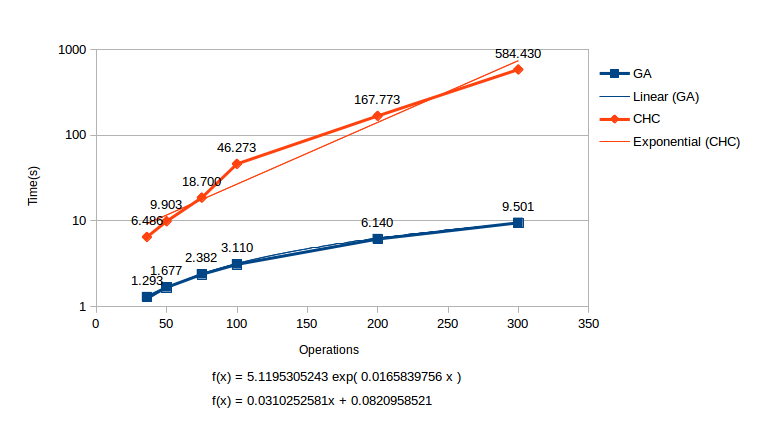
\includegraphics[width=0.5\textwidth]{./figuras/Graficas/GAvsCHCTime.png}
  \caption{$GA(27) vs. CHC(20)$}
  \label{grafica:tiempo}
\end{figure} 



\subsubsection{GA vs CHC}
Para entrar en contexto se sabe que los algoritmos genéticos (y en particular el algoritmo propuesto GA) enfatiza la importancia del operador de recombinación utilizándolo como operador primario mientras que se tiene un operador de mutación como mecanismo secundario secundario.
Sin embargo el CHC implementado que utiliza selección elitista y un operador de cruzamiento HUX no utiliza mutación. Esto lleva consigo a crear algún método que mantenga la diversidad; para ello se utiliza un mecanismo de re inicialización “secundario” que se aplica cuando se detecta convergencia en el conjunto de soluciones.
Esta comparación se realizará en igualdad de condiciones, con el objetivo de determinar si la presencia de un operador de mutación logra mejorar a gran escala los valores de fitness obtenidos. Básicamente la idea es contrastar dos aspectos importantes en cada algoritmo, a lo que refiere representación de la solución y la inclusión de un operador evolutivo secundario. El análisis consistirá en observar el impacto de dichos factores en la eficiencia computacional como la calidad de la solución. Se establecerá si el operador secundario es determinante en la calidad de la solución, así como la codificación puede tener un impacto positivo en la eficiencia computacional.
En resumen, la evaluación consistirá:
\begin{enumerate}
  \item Determinar si la diferencias entre los mecanismos utilizados para obtener diversidad en los algoritmos conllevan soluciones diferentes y ver cuáles de ellas obtuvo mejores soluciones globales. 
  \item Determinar si la codificación de la solución presenta alto impacto, en eficiencia computacional como en la calidad de las soluciones. Teniendo en cuenta que la codificación del algoritmo GA es un arreglo con la cantidad total de operaciones de una instancia del problema; en cambio CHC la codificación es binaria, la cual promete obtener con el operador de recombinación un conjunto de soluciones con la calidad esperada.
\end{enumerate}



\subsubsection{Análisis estadístico}
Los procedimientos a realizar para determinar la mejor calidad de un algoritmo frente a otro, dependerán de las distribuciones probabilísticas de los valores obtenidos para cada algoritmo.
Se utilizará tests paramétricos en el caso que ambos conjuntos de muestras de los algoritmos involucrados posean una distribución normal. Para ello se procede a realizar test de normalidad de D'Agostino, posteriormente se realizará test t-Student utilizando GNU-OCTAVE \cite{url:octave} para determinar si existen diferencias significativas entre las medias de los conjuntos en cuestión, en caso las instancias presenten un comportamiento bajo una distribución normal.
En caso de no tratarse de distribuciones normales, el procedimiento será análogo pero el objetivo es analizar la existencia de una diferencia significativa entre las medianas de los conjuntos de muestra, para ello se utiliza test de Mann-Witney(s-Student).

Una forma de poder comparar los algoritmos, puede ser simplemente observar los valores fitness hallados por un algoritmo y por el otro. Como podemos apreciar el algoritmo propuesto(GA), obtiene resultados notablemente mejores, es decir un fitness mejor en promedio e individual, que el CHC en todos los conjuntos de entradas testeados y para cualquier combinación paramétrica. Este resultado nos lleva a concluir que el algoritmo propuesto, en término de calidad de soluciones, obtiene mejoras a las soluciones buscadas.

\paragraph{Descripción Tablas}
El análisis estadístico será adjunta como parte de la entrega, esto se debe a la gran cantidad de tablas que presenta el mismo. Se trata del archivo \href{./Statistical\_Analysis.pdf}{Statistical\_Analysis.pdf}, el cual posee la siguiente información relevante:
\begin{itemize}
  \item Tablas fitness GA : En esta sección se presenta todos los valores de fitness encontrados en las 30 ejecuciones realizadas, así como el fitness promedio y el mínimo encontrado por cada instancia del problema propuesto.
  \item Tablas tiempos GA : Análogo al punto anterior, pero aplicado al tiempo de ejecución, incluye tiempo promedio para cada instancia al igual que el tiempo mínimo de ejecución.
  \item Tablas fitness CHC: Análogo al punto 1 pero aplicado al algoritmo CHC.
  \item Tablas tiempos CHC: Análogo al punto 2 pero aplicado al algoritmo CHC.
  \item Análisis del algoritmo GA: En esta sección se describen los datos obtenidos mediante en cada configuración de parámetros propuesto. Las columnas de las tablas para esta sección son $Instancia$ indica que instancia del problema corresponde los resultados; $F_{OPT}$ es el mejor valor de fitness conocido hasta el momento; $F_{BEST}$ es el mejor fitness encontrado mediante la ejecución del algoritmo; $F_{AVG}$ es el fitness promedio para la instancia dada; $\sigma$ es la desviación estándar; $T_{AVG}$ es el tiempo promedio de ejecución; $DA$ es el estádistico de D'Agostino para dicha instancia y $Normal$ describe dado el valor de $DA$ si la distribución es normal, es decir si $DA$ se encuentra en el intervalo  $[0.2662, 0.2866]$, dado $\alpha=0.05$ y un tamaño de muestra $N=30$.
  \item Análisis del algoritmo CHC: Análogo al item anterior pero aplicado a CHC.
  \item Comparación GA - CHC: Se trata de una tabla que compara los atributos de calidad entre ambos algoritmos; $F_{BEST}$ describe el mejor valor fitness encontrado por el algoritmo en cuestión, $F_{AVG}$ es el fitness promedio, $\sigma$ la desviación estándar para la instancia, y $T_{AVG}$ es el tiempo promedio de ejecución según el algoritmo en cuestión.
  \item s-student y t-student: Para en análisis estadístico se realizaron los test s-student para el caso de que las distribuciones de la instancia no sean normales, y t-student para el caso que ambas distribuciones lo sean. Para ello se describe mediante la columna $p-value$ el p-valor correspondiente al resultado del test, y la columna $Test$ indica el test realizado en ese caso. Se aplica s-student se aplica para analizar cual de las distribuciones presenta una mayor mediana, análogamente se utiliza t-student para analizar la diferencia entre la media de dos distribuciones normales, en este caso no interesa conocer quién posee la menor media, ya que el objetivo es minimizar el valor de fitness. Para el resultado de $p-valor$ lo interpretamos de la siguiente forma; la hipótesis nula que tomamos es la media de GA es mayor a la media de CHC, para el caso del test t-student, análogamente para el caso de las medianas pero considerando la hipótesis nula como la mediana de GA es mayor a la de CHC; entonces tenemos si $p-value < \alpha$, con $\alpha=0.05$, entonces rechazamos la hipótesis nula; y por lo tanto podemos deducir que efectivamente la media o la mediana de la muestra de la izquierda(GA) es menor que la muestra de la derecha(CHC), dependiendo del test realizado. En caso contrario no podemos afirmar que la hipótesis alternativa es cierta, pero en la mayoría de los casos se termina rechazando la hipótesis nula o el $p-valor$ es próximo a uno y terminamos aceptando la hipótesis alternativa.
  \item Caso 28: El caso 28 de prueba corresponde a la selección de la mejor configuración de parámetros encontrada, para el CHC corresponde a la configuración de parámetros $20$, mientras que para GA corresponde a la configuración $27$; para más detalles ver sección \ref{sec:parametros}.
  \item Todos los casos: La última tabla del documento en cuestión realiza una comparación a nivel macro, involucrando el fitness promedio($F_{AVG}$) y el tiempo promedio($T_{AVG}$) para cada configuración de parámetros. Para tener una noción sobre como evoluciona el comportamiento tanto a nivel de calidad de la solución promedio como en la eficiencia computacional expresada mediante el tiempo promedio de ejecución.
\end{itemize}

\subsubsection{GAP}
Se utilizó también un indicador que es utilizado para hacer comparaciones y saber cuan bueno es, en este caso, un algoritmo respecto a otro. El indicador es el GAP y lo definimos como $GAP=\frac{CHC-GA}{CHC}$. El estudio se hizo en base al algoritmo propuesto $GA$ y a $CHC$; el análisis se llevó a cabo para la calidad de las soluciones y para la eficiencia computacional en términos de tiempo de ejecución.

\label{tabla:gap}
\begin{table}
\begin{center}
    \begin{tabular}{| l | l | l|}
    \hline
    \textbf{Caso} & \textbf{$F_{AVG}$} & \textbf{$T_{AVG}$} \\ \hline
    1	& 0.0235	& 0.9263 \\ \hline
    2	& 0.0249	& 0.8961 \\ \hline
    3	& 0.0226	& 0.8854 \\ \hline
    4	& 0.0713	& 0.9082 \\ \hline
    5	& 0.0679	& 0.8985 \\ \hline
    6	& 0.0697	& 0.9011 \\ \hline
    7	& 0.0825	& 0.9066 \\ \hline
    8	& 0.0811	& 0.8955 \\ \hline
    9	& 0.0839	& 0.8899 \\ \hline
    10	& 0.0103	& 0.9583 \\ \hline
    11	& 0.0128	& 0.9513 \\ \hline
    12	& 0.0133	& 0.9467 \\ \hline
    13	& 0.0507	& 0.9555 \\ \hline
    14	& 0.0536	& 0.9496 \\ \hline
    15	& 0.0521	& 0.9423 \\ \hline
    16	& 0.0627	& 0.9521 \\ \hline
    17	& 0.0649	& 0.9499 \\ \hline
    18	& 0.0634	& 0.9396 \\ \hline
    19	& -0.0021	& 0.9771 \\ \hline
    20	& -0.0025	& 0.9742 \\ \hline
    21	& -0.0002	& 0.9709 \\ \hline
    22	& 0.0347	& 0.9769 \\ \hline
    23	& 0.0333	& 0.9747 \\ \hline
    24	& 0.0357	& 0.9698 \\ \hline
    25	& 0.0431	& 0.9750 \\ \hline
    26	& 0.0445	& 0.9717 \\ \hline
    27	& 0.0488	& 0.9695 \\ \hline
     
    \end{tabular}
\end{center}
\caption{GAP CHC vs GA}
\end{table}

Como se observa en la tabla \ref{tabla:gap}, existe una mejora del algoritmo propuesto respecto al CHC en término del promedio del  fitness hallado; donde en algunos casos se puede notar una mejora de hasta el $8\%$ $(0.08)$ como ser en el caso 9. Igual cabe aclarar que en ciertos casos como ser  19, 20 y 21 el CHC llegó a mejores promedios del fitness. La notable diferencia se encuentra aquí en los tiempos de ejecuciones de los algoritmos. Claramente el algoritmo propuesto llega a las soluciones en tiempos inalcanzables por el CHC, llegando a una diferencia del $97\%$ $(0.97)$ como ser los casos 19, 20 y 21.

\subsection{Ajuste de Parámetros}
Básicamente se realizó la ejecución de ambos algoritmos, con valores de parámetros que aporten calidad a la solución del problema. El análisis es exhaustivo por lo que para el algoritmo CHC se realizaron 27 ejecuciones de cada instancia del problema, combinando la probabilidad de cruzamiento ($P_{C}$), la probabilidad de reemplazo ($P_{R}$) y el tamaño de la población ($\#pob$).  Para el algoritmo GA se procedió con 27 ejecuciones también de las 20 instancias propuestas.


\subsubsection{Parámetros} \label{sec:parametros}
A continuación se listan los parámetros en cuestión:
\begin{enumerate}
  \item Tamaño de Población: El objetivo es trabajar con diversos tamaños de población y observar el comportamiento de los valores de fitness óptimos para cada caso. Se puede establecer en este punto una cota superior para el número de población para el cual, a mayor cardinalidad del conjunto los resultados presentan una variación despreciable. Para ello tomamos los siguientes valores $\#pob=\{50,100,200\}$.
  \item Probabilidad de mutación: Se alternó el valor de probabilidad de mutación entre valores razonables $P_{M}=\{0.1,0.05,0,01\}$. A partir de estos resultados se arriba a una conclusión respecto a la comparación de la mutación utilizado por GA y al operador secundario utilizado por CHC.
  \item Probabilidad de cruzamiento: Diversificar la población con una probabilidad adecuada es importante para lograr mejores resultados en menor tiempo, por ello se utilizaron probabilidades del conjunto $P_{C}=\{0.6,0.7,0.8\}$.
  \item Probabilidad de reemplazo: En el caso de existir convergencia, se utilizará un mecanismo de reemplazo de la población utilizando este parámetro de configuración, el mismo se aplicará a todos los individuos de la población, con la finalidad de generar una nueva población a partir de dichos parámetro. Se utilizaron los siguientes parámetros $P_{R}=\{0.5,0.7,0,9\}$.
\end{enumerate}


Observar que combinar todos los parámetros es una tarea costosa, de todas formas como estamos ante un análisis exhaustivo de los datos, se procedió a la ejecución de todas las combinaciones posibles, logrando un alto espectro de combinación de parámetros. Una vez que se obtuvo la mejor combinación posible se realizó una ejecución con un número de generaciones lo suficientemente elevado para llegar a mejores soluciones obtenidas anteriormente. Si bien se utilizó un numero de generaciones razonable para todas las instancias en cuestión, en algunas instancias no se llegó a la mejor solución conocida hasta el momento.  Es por ello que una vez definida la mejor combinación de parámetros, se procede a ponderar un número de generaciones elevado para aquellas instancias donde no se alcanzó el óptimo. Para cada combinación de parámetros se procedió a realizar una gráfica comparativa para cada algoritmo detallado. Consiste en representar dado un número de población, el valor de firness global a partir de los parámetros de cruzamiento y mutación, para el caso del algoritmo GA, en cambio para el algoritmo CHC se altera los valores de la probabilidad de cruzamiento  y la probabilidad de reemplazo.

Básicamente como se describió anteriormente, se realizaron 27 combinaciones de parámetros, cada una de ellas con 20 instancias del problema ejecutadas treinta veces para obtener un conjunto de datos razonables para realizar el análisis estadístico pertinente. En la tabla se resume todos los resultados logrados de las 27 combinaciones, comparando los dos algoritmos propuestos; los parámetros de calidad seleccionados fueron el tiempo promedio de procesamiento y el fitness promedio de todas las instancias. La tabla \ref{tabla:todoscasos} muestra dados los parámetros de configuración seleccionados, los ítems de calidad mencionados.
 
 
\npdecimalsign{.}
\nprounddigits{4}

\writetablecases
%%%TODO: SUBIR ARCHIVO DE TABLAS A GITHUB
Como se mencionó anteriormente, una vez se obtienen las posibles combinaciones con los parámetros mencionados, se deja a disposición todos los valores obtenidos para dicho caso. Cabe mencionar también que los datos de todos los casos citados en el presente informe se encuentran adjuntos en el archivo \href{./Statistical\_Analysis.pdf}{Statistical\_Analysis.pdf}, de esta forma se agrega información extra de los resultados obtenidos, con los parámetros correspondientes. 
Se puede observar que el mejor fitness promedio se obtuvo en el caso 27, donde los parámetros son $P_{C} = 0.8$ , $P_{M} = 0.1$ y $\#ind=200$; es decir, con la mayor probabilidad de cruzamiento y mutación dentro de las probabilidades designadas. Cabe aclarar también que el mejor promedio de fitness se obtuvo con la mayor cantidad de individuos. Si observamos detenidamente el archivo \href{./Statistical\_Analysis.pdf}{Statistical\_Analysis.pdf} podemos ver que a igual $P_{C}$ y $P_{M}$ en caso del algoritmo GA y a mayor $\#ind$ el promedio de fitness mejora; al igual el CHC cuando fijamos $P_{C}$ y $P_{R}$ a mayor $\#ind$ el promedio de fitness mejora. Esto nos lleva a concluir que la cantidad de individuos efectivamente es un factor determinante en la búsqueda del mejor fitness.
Para el caso 27 mencionado anteriormente se adjunta la tabla de valores [\ref{tabla:mejorcaso}] correspondiente a las ejecuciones para cada instancia, así como el tiempo, fitness promedio, el mejor valor de fitness obtenido de las ejecuciones y el valor DA estadístico de D’Agostino que se obtuvo en cada caso, el cual determina si los datos son normales, para este caso se tomó como referencia $\alpha = 0.05$ y un tamaño de muestra $N=30$, para que la muestra sea normal, el valor estadístico DA para cada caso debe pertenecer al intervalo $[0.2662, 0.2866]$, caso contrario se trata de una muestra que no sigue dicha distribución probabilística. 
Otro dato a tener en cuenta es si con el algoritmo propuesto se arriba a la mejor solución encontrada hasta el momento. Para el caso 27 cuya configuración de parámetros reporta mejor fitness promedio, se arriba a las mejores soluciones para las instancias listadas a continuación:

\begin{itemize}
  \item la01
  \item la05
  \item la06
  \item mt06
  \\
\end{itemize}
Para las demás se pretende realizar una ejecución que involucre un mayor número de generaciones, con al finalidad de aproximarse o alcanzar los valores óptimos conocidos hasta el momento.

Esto se debe a que la cantidad de operaciones para estas instancias son mayores o iguales a 100, para remediar este caso se ejecutará 30 veces cada instancia mencionada con un número de generaciones mayor, en este caso 5000 en contraste a 1000 utilizadas en todos los casos. De esta forma, ejecutando el algoritmo con la mejor configuración de parámetros, puede mejorarse los resultados a un costo computacional lineal.
La tabla \ref{tabla:5000gen}, muestra los valores de fitness óptimos obtenidos por el algoritmo GA.


\begin{table}[!htb]
\begin{center}

  \begin{tabular}{|l | r | r | N{5}{4}| N{5}{4}|}
  \hline

  \multicolumn{1}{|l}{Instancia}&
  \multicolumn{1}{|c}{$F_{OPT}$}&
  \multicolumn{1}{|c}{$F_{BEST}$}&
  \multicolumn{1}{|c}{$F_{AVG}$}&
  \multicolumn{1}{|c|}{$T_{AVG}$}
  \tabularnewline
  \hline
  
  
  abz5 &  1234 & 1263 & 1311.3 & 15.72763 \tabularnewline
abz6 &  943 & 947 & 981.9 & 15.55253 \tabularnewline
abz7 &  656 & 737 & 779.7666666666667 & 47.82475666666667 \tabularnewline
abz8 &  665 & 758 & 802.2 & 47.63549666666666 \tabularnewline
abz9 &  679 & 800 & 834.1666666666666 & 47.84549666666666 \tabularnewline
la01 &  666 & 666 & 673.3333333333334 & 8.322461666666667 \tabularnewline
la02 &  655 & 655 & 680.5666666666667 & 8.537937333333334 \tabularnewline
la03 &  597 & 606 & 631.9333333333333 & 8.522019333333335 \tabularnewline
la04 &  590 & 590 & 606.8666666666667 & 8.557941333333334 \tabularnewline
la05 &  593 & 593 & 593 & 8.581372999999999 \tabularnewline
la06 &  926 & 926 & 926 & 11.89785333333333 \tabularnewline
la29 &  1153 & 1276 & 1347.3 & 30.67480333333333 \tabularnewline
mt06 &  55 & 55 & 55.16666666666666 & 6.474112666666667 \tabularnewline
mt10 &  930 & 1005 & 1056.6 & 15.68444666666667 \tabularnewline
mt20 &  1165 & 1228 & 1315.666666666667 & 15.75459333333333 \tabularnewline
orb1 &  1059 & 1119 & 1195.033333333333 & 15.82228 \tabularnewline
orb2 &  888 & 909 & 958.3333333333334 & 15.84372666666667 \tabularnewline
orb3 &  1005 & 1086 & 1173.066666666667 & 15.50103 \tabularnewline
orb4 &  1005 & 1046 & 1088.833333333333 & 15.59161 \tabularnewline
orb5 &  887 & 946 & 1012.433333333333 & 15.62667333333333 \tabularnewline

  
  
  \hline
  \end{tabular}
  
\end{center}
\caption{$P_{C}=0.8, P_{M}=0.1, \#Individuos=200, \#gen=5000$}
\label{tabla:5000gen}
\end{table}



Observar que incrementando el número de generaciones a 5000 los resultados obtenidos para las instancias se aproximaron al óptimo, pero no se alcanzó en algunas instancias, esto se debe a la complejidad de las instancias los resultados más alejados del óptimo se encuentran en las instancias $abz7$, $abz8$ y $abz9$, donde la cantidad de operaciones es de $300$. Para estos casos se debe incrementar el número de generaciones, hasta converger a la solución óptima, si bien este procedimiento agrega un costo extra a nivel computacional, podemos asumirlo para las instancias que poseen más operaciones, como las mencionadas anteriormente.

Para el caso de CHC, se ejecutaron todas las instancias con un número de generaciones de $5000$, en este caso se mejoraron algunos óptimos de instancias, y el valor de fitness promedio al igual que en el caso de GA se redujo notoriamente. Sin embargo al aumentar el número de generaciones el algoritmo GA se comportó en la totalidad de las instancias mejor que CHC, que en una gran cantidad de casos en los tests de configuración de parámetros obtuvo mejores resultados individuales en algunas instancias.
Los resultados obtenidos en la ejecución de 5000 generaciones para CHC se presentan en la tabla \ref{tabla:5000genCHC}, a pesar de ejecutar con un mayor número de generaciones los resultados obtenidos con CHC superaron con una diferencia mínima los resultados obtenidos en el caso 20, con un costo computacional 5 veces superior. Esto se debe claramente a que la representación binaria en este problema específico conlleva a que los resultados converjan de forma lenta, el tamaño de las soluciones son demasiado complejas por lo tanto se requiere un número de generaciones muy por encima del sugerido para obtener valores semejantes al GA.
Pero esto no quiere decir que CHC presente un comportamiento insuficiente, basta ver instancias individuales en las cuales CHC supera ampliamente a GA como ser en el caso $20$ donde incluso en instancias de gran tamaño como ser $orb1$, $orb2$, $la29$ y $abz6$. Instancias como $la02$ CHC en casi todos los casos supera a GA, si tomamos como atributo de calidad el fitness promedio estamos ponderando el promedio de los casos, y no las instancias individuales, basta ver los mejores fitness en instancias individuales para deducir que en algunos casos CHC se comporta de mejor forma que GA. Sin embargo cuando ponderamos mayor número de generaciones, GA converge más rápido al óptimo que CHC en prácticamente todas las instancias.
Podemos decir que el desempeño de CHC en instancias $la$ supera levemente a GA, con lo cual podemos tomar como referencia este algoritmo para las instancias de este tipo cuando trabajamos con un orden de generaciones moderado(1000).
Como se mencionó anteriormente no se pueden extraer conclusiones sobre el valor promedio de fitness, sin embargo cuando combinamos la calidad de las soluciones y la eficiencia computacional, GA en el segundo ítem tiene un mejor desempeño, de tal forma que se podría ejecutar con dicho algoritmo un número de generaciones lo suficientemente extenso como para alcanzar la mayoría de las soluciones óptimas en el mismo tiempo que se ejecuta CHC en un número bajo de generaciones.
Otro punto interesante que puedo resultar relevante para el problema; el algoritmo CHC brinda una desviación estándar en todos los casos más ajustada que el algoritmo GA, esto acota el espacio y puede ser útil cuando queremos que dicha desviación sea minimizada, caso contrario es conveniente utilizar GA puesto que la desviación estándar para ese caso presenta un intervalo mayor, en el cual las soluciones varían. Puede ser un criterio a tener en cuenta cuando se selecciona el algoritmo para el problema.


\begin{table}[!htb]
\begin{center}
  \begin{tabular}{|l | r | r | N{5}{4}| N{5}{4}|}
  \hline

  \multicolumn{1}{|l}{Instancia}&
  \multicolumn{1}{|c}{$F_{OPT}$}&
  \multicolumn{1}{|c}{$F_{BEST}$}&
  \multicolumn{1}{|c}{$F_{AVG}$}&
  \multicolumn{1}{|c|}{$T_{AVG}$}
  \tabularnewline
  \hline
  
  
  abz5 &  1234 & 1351 & 1413.633333333333 & 201.4588333333333 \tabularnewline
abz6 &  943 & 975 & 1014.833333333333 & 206.7888 \tabularnewline
abz7 &  656 & 884 & 921.7 & 2354.218666666667 \tabularnewline
abz8 &  665 & 901 & 935.7 & 2365.644 \tabularnewline
abz9 &  679 & 909 & 950.5 & 2302.667666666667 \tabularnewline
la01 &  666 & 688 & 694.1 & 47.67087 \tabularnewline
la02 &  655 & 664 & 672.0333333333333 & 64.77999333333334 \tabularnewline
la03 &  597 & 622 & 640.6666666666666 & 46.69001666666666 \tabularnewline
la04 &  590 & 613 & 631.9333333333333 & 48.94486333333334 \tabularnewline
la05 &  593 & 593 & 593 & 50.55932333333334 \tabularnewline
la06 &  926 & 926 & 926.1666666666666 & 88.17637999999999 \tabularnewline
la29 &  1153 & 1448 & 1516.866666666667 & 774.1625 \tabularnewline
mt06 &  55 & 55 & 55 & 36.55735666666666 \tabularnewline
mt10 &  930 & 1087 & 1119.233333333333 & 215.0965 \tabularnewline
mt20 &  1165 & 1341 & 1396.266666666667 & 135.5221 \tabularnewline
orb1 &  1059 & 1215 & 1269.066666666667 & 225.2851 \tabularnewline
orb2 &  888 & 948 & 998.1666666666666 & 217.9525333333333 \tabularnewline
orb3 &  1005 & 1152 & 1219.166666666667 & 220.8019333333334 \tabularnewline
orb4 &  1005 & 1099 & 1149.833333333333 & 227.7694 \tabularnewline
orb5 &  887 & 1023 & 1075.133333333333 & 224.7588666666666 \tabularnewline

  
  
  \hline
  \end{tabular}
\end{center}
\caption{$P_{C}=0.7, P_{R}=0.5, \#Individuos=200, \#gen=5000$}
\label{tabla:5000genCHC}
\end{table}

\begin{enumerate}
  \item En primer lugar, la representación seleccionada para GA es más eficiente computacionalmente que en el caso de CHC, esto se explicó anteriormente, pero con los datos experimentales se confirma la hipótesis inicial.
  \item El mecanismo de reparación para que una solución sea válida en el algoritmo CHC es costosa, esto se debe a la representación de la solución, lo cual implica un proceso de 'local harmonization', el cual implica la construcción de matrices de amplias proporciones para verificar si la solución es factible, y en caso de no ser repararla. Es importante destacar que forzar soluciones provee mejores desempeños, para ello se adjunta documento que describe la eficiencia de CHC forzando soluciones que satisfacen el problema en lugar de invalidar la solución\cite{url:binaria}.
  \item Sin dudas la representación es el principal factor que lleva a CHC a obtener resultados por debajo del algoritmo GA, ya que CHC requiere que la codificación de la solución sea binaria, esto repercute en la cantidad de bits que se deben dedicar para representar la solución, al tratarse de una relación entre operaciones, el tamaño de la solución es extensa, lo cual a nivel computacional requiere un tiempo de procesamiento mayor al del algoritmo GA. Esto también tiene un impacto directo cuando se aplica operadores evolutivos como ser cruzamiento y reemplazo generacional en caso de convergencia.
\end{enumerate}


\subsection{Gráficas}
Para la mejor representación de los datos, se adjunta para todos los casos propuestos de combinación de parámetros discriminado por $\#individuos$, se presentan las gráficas comparativas entre CHC y GA, comparando los valores fitness promedio para todas las instancias del problema.

En la figura \ref{fig:comp50} se obtiene la comparación de fitness promedio entre los algoritmos propuestos con $\#individuos=50$, en función de los parámetros de mutación y cruzamiento. De forma análoga en la figura \ref{fig:comp100} para $\#individuos=100$ y la figura \ref{fig:comp200} para $\#individuos=200$.


\begin{figure}[]
  \centering
    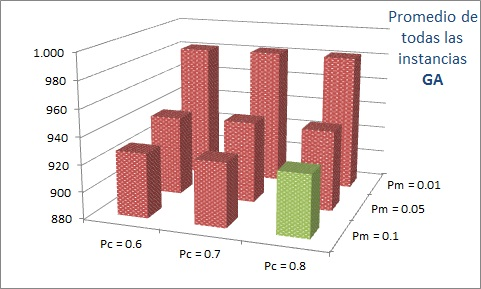
\includegraphics[width=0.5\textwidth]{./figuras/Graficas/Comparacion/GA-50IND.jpg}
    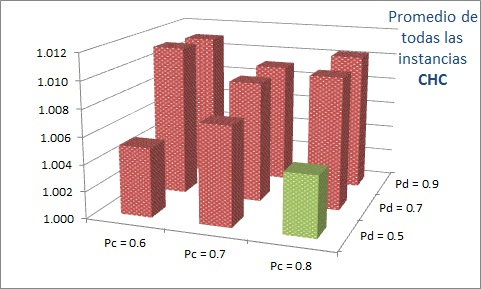
\includegraphics[width=0.5\textwidth]{./figuras/Graficas/Comparacion/CHC-50IND.jpg}
  \caption{$\#individuos=50$}
  \label{fig:comp50}
\end{figure} 


\begin{figure}[]
  \centering
    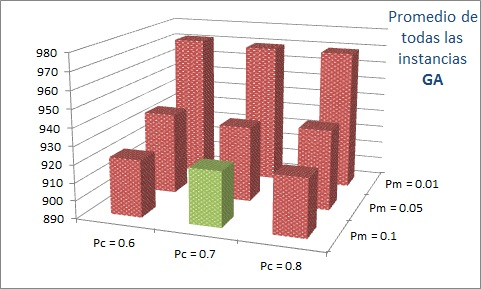
\includegraphics[width=0.5\textwidth]{./figuras/Graficas/Comparacion/GA-100IND.jpg}
    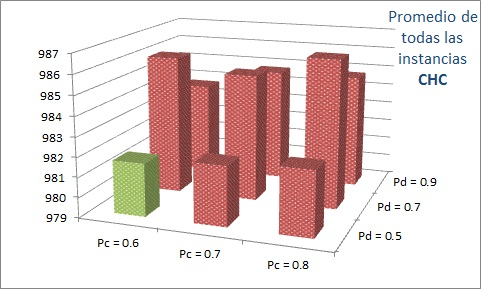
\includegraphics[width=0.5\textwidth]{./figuras/Graficas/Comparacion/CHC-100IND.jpg}
  \caption{$\#individuos=100$}
  \label{fig:comp100}
\end{figure} 


\begin{figure}[]
  \centering
    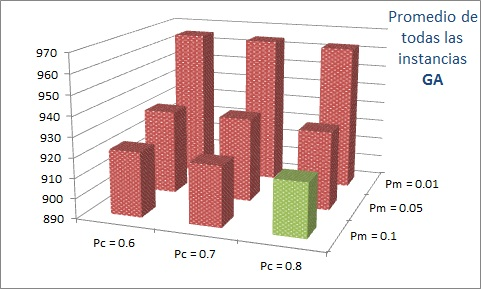
\includegraphics[width=0.5\textwidth]{./figuras/Graficas/Comparacion/GA-200IND.jpg}
    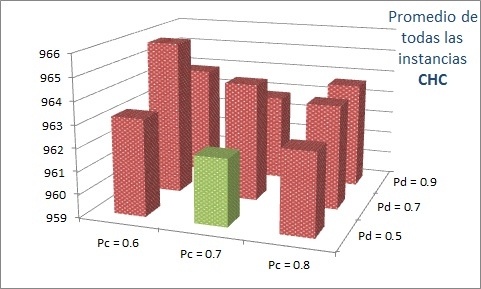
\includegraphics[width=0.5\textwidth]{./figuras/Graficas/Comparacion/CHC-200IND.jpg}
  \caption{$\#individuos=200$}
  \label{fig:comp200}
\end{figure} 



\newpage
\section{Conclusiones}
En el presente proyecto se plantea un algoritmo evolutivo que para el conjunto de casos de entradas testeado, es realmente eficiente computacionalmente hablando si lo comparamos con otro tipo de algoritmo; lo cual era uno de los principales objetivos planteados. El algoritmo consigue obtener una calidad elevada de soluciones al problema y conjunto a lo dicho anteriormente, en un tiempo más que satisfactorio.
Teniendo en cuenta la probabilidad de mutación ($P_{M}$), la probabilidad de cruzamiento ($P_{C}$) y la cardinalidad de individuos ($\#ind$), podemos concluir que la mejor combinación de parámetros en la que se obtiene un mejor promedio de fitness es $P_{M}=0.1$, $P_{C}=0.8$ y a mayor $\#ind$ mejores resultados, para este caso $\#ind=200$.
Los algoritmos evolutivos contribuyen con los problemas considerados NP-difíciles brindando alternativas para llegar a soluciones cotizadas como ‘muy buenas’ en un tiempo bajo si es comparado con otras técnicas. De hecho podemos remarcar que el algoritmo propuesto presenta una mejora significativa en términos de tiempos, comparándolo con un algoritmo que utiliza la misma técnica, pero con una variante bastante importante, que es la no utilización de mutación. 
Podemos extraer una conclusión importante sobre la utilización de algoritmos evolutivos para la resolución de problemas; no es fácil predecir qué parámetros o criterios utilizar para solucionar el problema de forma satisfactible. 
Una conclusión importante es que el operador de mutación, agrega diversidad al problema y genera mejores resultados, basta comparar casos de prueba donde la probabilidad de mutación es menor, y los resultados son evidentes, a mayor diversidad, mejor es fitness promedio, por ende contribuye a obtener mejores soluciones globales. Para este tipos de problemas, la diversidad es sin lugar a dudas el factor determinante para obtener mejores soluciones, tanto en el algoritmo GA como CHC.
A medida que se obtienen los resultados, se concreta la hipótesis primaria del problema, a mayor diversidad las soluciones mejoran, esto quedó plasmado cuando se alteraron los parámetros con el fin de brindar mayor diversidad al problema. En ambos algoritmos la hipoótesis es válida obteniendo mejoras notorias en el algoritmo CHC a medida que se ajustan los parámetros para obtener mayor diversidad, es decir, que la probabilidad de cruzamiento, mutación y reemplazo en el caso de CHC, así como la cantidad de individuos sea lo mayor posible.
Si bien el conocimiento global del problema es un reto difícil de asumir, ya que el problema ha sido estudiado por muchos años, no se pretendía sobrepasar las mejores marcas, pero sí lograr mediante una propuesta computacionalmente eficiente arribar a resultados semejantes a los conseguidos hasta el momento.
Se concluye que a pesar de no colmar todos los objetivos como ser superar valores óptimos, la experiencia implementando una solución a JSSP mediante algoritmos evolutivos, conduce que su utilización es completamente válida para cualquier otro problema NP-difícil. Por tanto, la utilización de este tipo de algoritmos es una buena estrategia a considerar en todos los problemas de esta índole.

\onecolumn

\begin{sidewaystable}
\section{Anexo}

\captionsetup{format=myformat, labelsep=newline}

\begin{center}
  \begin{tabular}{|l | r | r | N{5}{4} | n{5}{4} | n{5}{4} | N{5}{4} | l|}
  \hline

  \multicolumn{1}{|l}{Instancia}&
  \multicolumn{1}{|c}{$F_{OPT}$}&
  \multicolumn{1}{|c}{$F_{BEST}$}&
  \multicolumn{1}{|c}{$F_{AVG}$}&
  \multicolumn{1}{|c}{$\sigma$}&
  \multicolumn{1}{|c}{$T_{AVG}$}&
  \multicolumn{1}{|c}{$DA$}&
  \multicolumn{1}{|c|}{Normal}\tabularnewline
  \hline

  abz5 &  1234 & 1268 & 1327.866666666667 & 33.0391014136617 & 3.119543666666666 & 0.2732788878197346&$ Si $ \tabularnewline
abz6 &  943 & 948 & 997.4666666666667 & 35.66392512827991 & 3.129972 & 0.2669675611101284&$ Si $ \tabularnewline
abz7 &  656 & 783 & 815.9 & 15.72121708604861 & 9.532662333333334 & 0.2843644694355653&$ Si $ \tabularnewline
abz8 &  665 & 774 & 829.3666666666667 & 27.58802074975458 & 9.471156333333333 & 0.2790865105650226&$ Si $ \tabularnewline
abz9 &  679 & 813 & 858.3333333333334 & 23.56315391076123 & 9.497831666666666 & 0.2832576856953026&$ Si $ \tabularnewline
la01 &  666 & 666 & 682.3666666666667 & 17.48043350593903 & 1.670503 & 0.2633102763849633&$ No $ \tabularnewline
la02 &  655 & 662 & 691.3 & 23.47218211699401 & 1.679026666666667 & 0.2675744216814164&$ Si $ \tabularnewline
la03 &  597 & 617 & 637.7 & 16.92759088982639 & 1.680406333333333 & 0.2640987476984923&$ No $ \tabularnewline
la04 &  590 & 598 & 615.4666666666667 & 10.0323919824182 & 1.673995333333333 & 0.2828615331967684&$ Si $ \tabularnewline
la05 &  593 & 593 & 593 & 0 & 1.682632& * &$ Si $ \tabularnewline
la06 &  926 & 926 & 926 & 0 & 2.381599& * &$ Si $ \tabularnewline
la29 &  1153 & 1320 & 1381.733333333333 & 36.63143762155973 & 6.140359666666667 & 0.2757497867123298&$ Si $ \tabularnewline
mt06 &  55 & 55 & 56.4 & 1.665332799572906 & 1.2925 & 0.2588738486515576&$ No $ \tabularnewline
mt10 &  930 & 1010 & 1071.2 & 30.31435303614445 & 3.069862333333333 & 0.281458166435189&$ Si $ \tabularnewline
mt20 &  1165 & 1258 & 1339.233333333333 & 47.1604942957792 & 3.124276 & 0.2830641333129369&$ Si $ \tabularnewline
orb1 &  1059 & 1135 & 1219.5 & 38.28206716814893 & 3.079718 & 0.2808828930409536&$ Si $ \tabularnewline
orb2 &  888 & 911 & 968.3333333333334 & 29.62806477349174 & 3.125906666666666 & 0.2642389554883586&$ No $ \tabularnewline
orb3 &  1005 & 1106 & 1181.833333333333 & 40.3212791904666 & 3.083039333333334 & 0.273015478535118&$ Si $ \tabularnewline
orb4 &  1005 & 1041 & 1105.933333333333 & 36.71959815805299 & 3.128086666666666 & 0.2803226029061514&$ Si $ \tabularnewline
orb5 &  887 & 942 & 1034.233333333333 & 42.44893664418724 & 3.133871 & 0.2822345270030719&$ Si $ \tabularnewline


  \hline
  \end{tabular}
\end{center}


  \caption{
  $P_{C}=0.8, P_{M}=0.1, \#Individuos=200$ \newline
  (*) $\sigma=0$  No definido DA, se asume Normalidad.
  }




\begin{comment}
  \centering
  \caption{$P_{C}=0.7, P_{M}=0.05, \#Individuos=200$}
  \begin{tabular}{|l|r|r|n{5}{4}|n{5}{4}|n{5}{4}|n{5}{4}|n{5}{4}|n{5}{4}|n{5}{4}|n{5}{4}|l|l|}
  \hline
  \multicolumn{1}{|l}{}&
  \multicolumn{2}{|c}{$F_{BEST}$}&
  \multicolumn{2}{|c}{$F_{AVG}$}&
  \multicolumn{2}{|c}{$\sigma$}&
  \multicolumn{2}{|c}{$T_{AVG}$}&
  \multicolumn{2}{|c}{DA}&
  \multicolumn{2}{|c|}{Normal}
  \tabularnewline
  \multicolumn{1}{|l}{Instancia}&
  \multicolumn{1}{|c}{GA}&
  \multicolumn{1}{c}{CHC}&
  \multicolumn{1}{|c}{GA}&
  \multicolumn{1}{c}{CHC}&
  \multicolumn{1}{|c}{GA}&
  \multicolumn{1}{c}{CHC}&
  \multicolumn{1}{|c}{GA}&
  \multicolumn{1}{c}{CHC}&
  \multicolumn{1}{|c}{GA}&
  \multicolumn{1}{c}{CHC}&
  \multicolumn{1}{|c}{GA}&
  \multicolumn{1}{c|}{CHC}
  \tabularnewline
  \hline
  abz5 &  1268 & 1348 & 1327.866666666667 & 1399.4 & 33.0391014136617 & 25.24229255304148 & 3.119543666666666 & 47.20402666666666\tabularnewline
abz6 &  948 & 989 & 997.4666666666667 & 1018.133333333333 & 35.66392512827991 & 15.52145468554914 & 3.129972 & 44.56548\tabularnewline
abz7 &  783 & 891 & 815.9 & 932.9333333333333 & 15.72121708604861 & 19.15538798586155 & 9.532662333333334 & 582.688\tabularnewline
abz8 &  774 & 924 & 829.3666666666667 & 953.9 & 27.58802074975458 & 15.30653455227538 & 9.471156333333333 & 662.3351333333334\tabularnewline
abz9 &  813 & 907 & 858.3333333333334 & 950.9 & 23.56315391076123 & 18.17021372099587 & 9.497831666666666 & 572.3139666666666\tabularnewline
la01 &  666 & 688 & 682.3666666666667 & 695.7666666666667 & 17.48043350593903 & 4.63812701661158 & 1.670503 & 9.812591333333334\tabularnewline
la02 &  662 & 657 & 691.3 & 673.3666666666667 & 23.47218211699401 & 11.28563492035586 & 1.679026666666667 & 9.338791333333335\tabularnewline
la03 &  617 & 617 & 637.7 & 639.6333333333333 & 16.92759088982639 & 12.2133351528383 & 1.680406333333333 & 9.350614333333334\tabularnewline
la04 &  598 & 613 & 615.4666666666667 & 644.3 & 10.0323919824182 & 21.2354263751245 & 1.673995333333333 & 9.310611666666667\tabularnewline
la05 &  593 & 593 & 593 & 593 & 0 & 0 & 1.682632 & 10.251382\tabularnewline
la06 &  926 & 926 & 926 & 926.3 & 0 & 0.8999999999999997 & 2.381599 & 18.59616666666667\tabularnewline
la29 &  1320 & 1427 & 1381.733333333333 & 1512.433333333333 & 36.63143762155973 & 38.57519352583413 & 6.140359666666667 & 163.4414\tabularnewline
mt06 &  55 & 55 & 56.4 & 55.03333333333333 & 1.665332799572906 & 0.1795054935711501 & 1.2925 & 6.774292666666667\tabularnewline
mt10 &  1010 & 1064 & 1071.2 & 1125.166666666667 & 30.31435303614445 & 24.81139970972125 & 3.069862333333333 & 47.90960333333334\tabularnewline
mt20 &  1258 & 1353 & 1339.233333333333 & 1411.6 & 47.1604942957792 & 30.71546841576733 & 3.124276 & 29.72073333333333\tabularnewline
orb1 &  1135 & 1196 & 1219.5 & 1274.833333333333 & 38.28206716814893 & 33.3187468084994 & 3.079718 & 44.55316\tabularnewline
orb2 &  911 & 958 & 968.3333333333334 & 995.2333333333333 & 29.62806477349174 & 20.72145962254804 & 3.125906666666666 & 45.69357\tabularnewline
orb3 &  1106 & 1170 & 1181.833333333333 & 1234 & 40.3212791904666 & 30.3271055877961 & 3.083039333333334 & 43.98836\tabularnewline
orb4 &  1041 & 1106 & 1105.933333333333 & 1153.066666666667 & 36.71959815805299 & 19.61450710287896 & 3.128086666666666 & 45.91886666666667\tabularnewline
orb5 &  942 & 1024 & 1034.233333333333 & 1084.466666666667 & 42.44893664418724 & 30.97066712588255 & 3.133871 & 44.23114666666667\tabularnewline

  \hline
  \end{tabular}
  
\end{comment}  
\label{tabla:mejorcaso}
\end{sidewaystable}
  
\newpage
\twocolumn
\bibliographystyle{plain}
\bibliography{bibliografia}

%\end{table}




\begin{comment}
\noindent\resizebox{\textwidth}{5cm}{
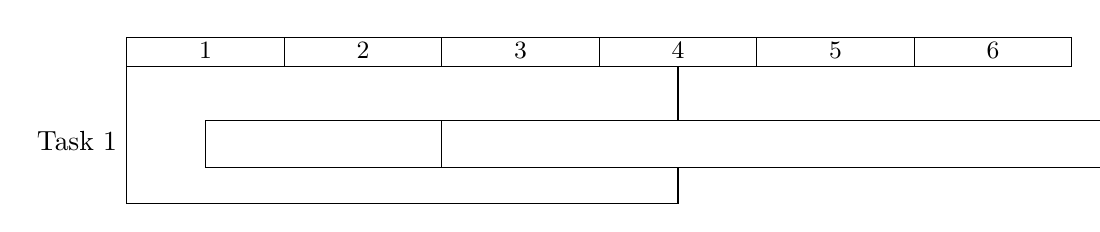
\begin{tikzpicture}[x=.2cm, y=1cm]

\begin{ganttchart}[x unit=1cm, y unit title=.6cm, y unit chart=1.5cm]{0}{6}
\gantttitlelist{1,...,6}{2} \\
\ganttbar{Task 1}{1}{12}
\ganttbar{}{1}{3}

\end{ganttchart}
\end{tikzpicture}
}

\begin{ganttchart}[x unit=.015cm, y unit title=.6cm, y unit chart=1.5cm]{0}{1500}
\gantttitle{Title 1}{1000} \\
\gantttitle{Title 2}{1000} \\
\ganttbar{}{10}{560} \\
\ganttbar{}{40}{650}
\end{ganttchart}

\end{comment}

\begin{comment}
\definecolor{red}{RGB}{255,0,0}
\definecolor{blue}{RGB}{0,153,255}
\definecolor{yellow}{RGB}{234,187,0}
\definecolor{green}{RGB}{0,255,0}
\definecolor{fucsia}{RGB}{255,0,255}
\definecolor{aqua}{RGB}{0,255,255}
\definecolor{black}{RGB}{0,0,0}
\definecolor{white}{RGB}{255,255,255}
\definecolor{orange}{RGB}{252,149,31}
\definecolor{gray}{RGB}{123,123,123}


\newganttchartelement{foobar}{
foobar/.style={
%shape=rounded rectangle,
%inner sep=0pt,
draw=blue!50!black,
%very thick,
%top color=white,
bottom color=blue!50
}
}

\newganttchartelement{redbar}{
redbar/.style={
draw=red!50!black,
bottom color=red!50
}
}

\newganttchartelement{bluebar}{
bluebar/.style={
draw=blue!50!black,
bottom color=blue!50
}
}
\newganttchartelement{yellowbar}{
yellowbar/.style={
draw=yellow!50!black,
bottom color=yellow!50
}
}



\newganttchartelement{greenbar}{
greenbar/.style={
draw=green!50!black,
bottom color=green!50
}
}

\newganttchartelement{fucsiabar}{
fucsiabar/.style={
draw=fucsia!50!black,
bottom color=fucsia!50
}
}

\newganttchartelement{aquabar}{
aquabar/.style={
draw=aqua!50!black,
bottom color=aqua!50
}
}

\newganttchartelement{blackbar}{
blackbar/.style={
draw=black!50!black,
bottom color=black!50
}
}

\newganttchartelement{whitebar}{
whitebar/.style={
draw=white!50!black,
bottom color=white!50
}
}

\newganttchartelement{orangebar}{
orangebar/.style={
draw=orange!50!black,
bottom color=orange!50
}
}

\newganttchartelement{graybar}{
graybar/.style={
draw=gray!50!black,
bottom color=gray!50
}
}

\begin{ganttchart}[x unit=.2cm, y unit title=.6cm, y unit chart=1.5cm]{0}{60}
\ganttyellowbar{Job 0}{0}{0}
\ganttredbar{}{1}{3}
\ganttbluebar{}{16}{21}
\ganttgreenbar{}{30}{36}
\ganttaquabar{}{42}{44}
\ganttfucsiabar{}{49}{54}\\
\ganttbluebar{Job 1}{0}{7}
\ganttyellowbar{}{8}{12}
\ganttfucsiabar{}{13}{22}
\ganttaquabar{}{28}{37}
\ganttredbar{}{38}{47}
\ganttgreenbar{}{48}{51}\\
\ganttyellowbar{Job 2}{1}{5}
\ganttgreenbar{}{6}{9}
\ganttaquabar{}{10}{17}
\ganttredbar{}{18}{26}
\ganttbluebar{}{27}{27}
\ganttfucsiabar{}{38}{44}\\
\ganttbluebar{Job 3}{8}{12}
\ganttredbar{}{13}{17}
\ganttyellowbar{}{22}{26}
\ganttgreenbar{}{27}{29}
\ganttfucsiabar{}{30}{37}
\ganttaquabar{}{45}{53}\\
\ganttyellowbar{Job 4}{13}{21}
\ganttbluebar{}{22}{24}
\ganttfucsiabar{}{25}{29}
\ganttaquabar{}{38}{41}
\ganttredbar{}{48}{50}
\ganttgreenbar{}{52}{52}\\
\ganttbluebar{Job 5}{13}{15}
\ganttgreenbar{}{16}{18}
\ganttaquabar{}{19}{27}
\ganttredbar{}{28}{37}
\ganttfucsiabar{}{45}{48}
\ganttyellowbar{}{49}{49}\\

\end{ganttchart}
\end{comment}


\end{document}
